
\begin{figure}[h]
\centering
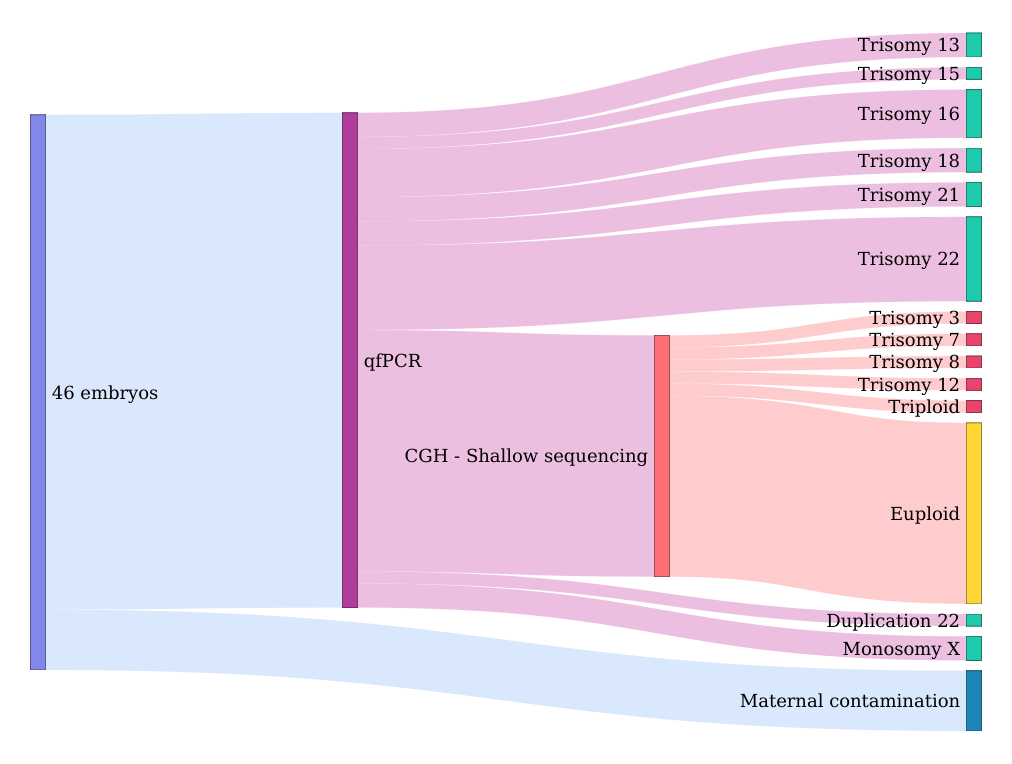
\includegraphics[width=0.7\textwidth]{fig/ibelieve.png}
\caption{\textbf{Pre-sequencing screening outcome.} }
\label{fig:presequencing}
\end{figure}

\begin{figure}[ht]
\centering
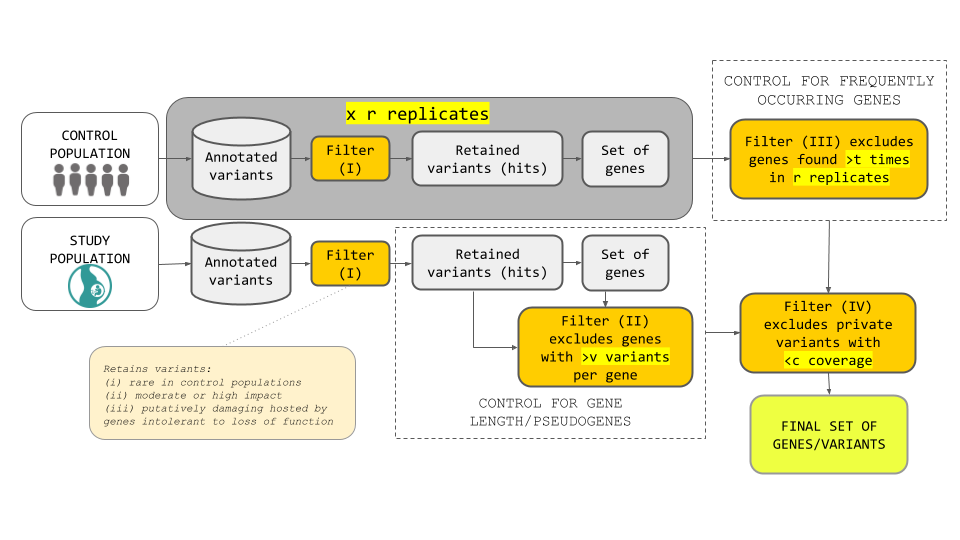
\includegraphics[width=\linewidth]{fig/pipeonly.png}
\caption{\textbf{Overview of the pipeline for prioritization for sequencing (A) Main steps.} Samples are first screened for the quality of DNA and maternal contamination and then analyzed for aneuploidies. \textbf{(B) Outcomes of the pipeline.} We estimate that 18\% of samples goes to sequencing....} 
\label{fig:pipeline}
\end{figure}

\begin{figure}[ht]
\centering
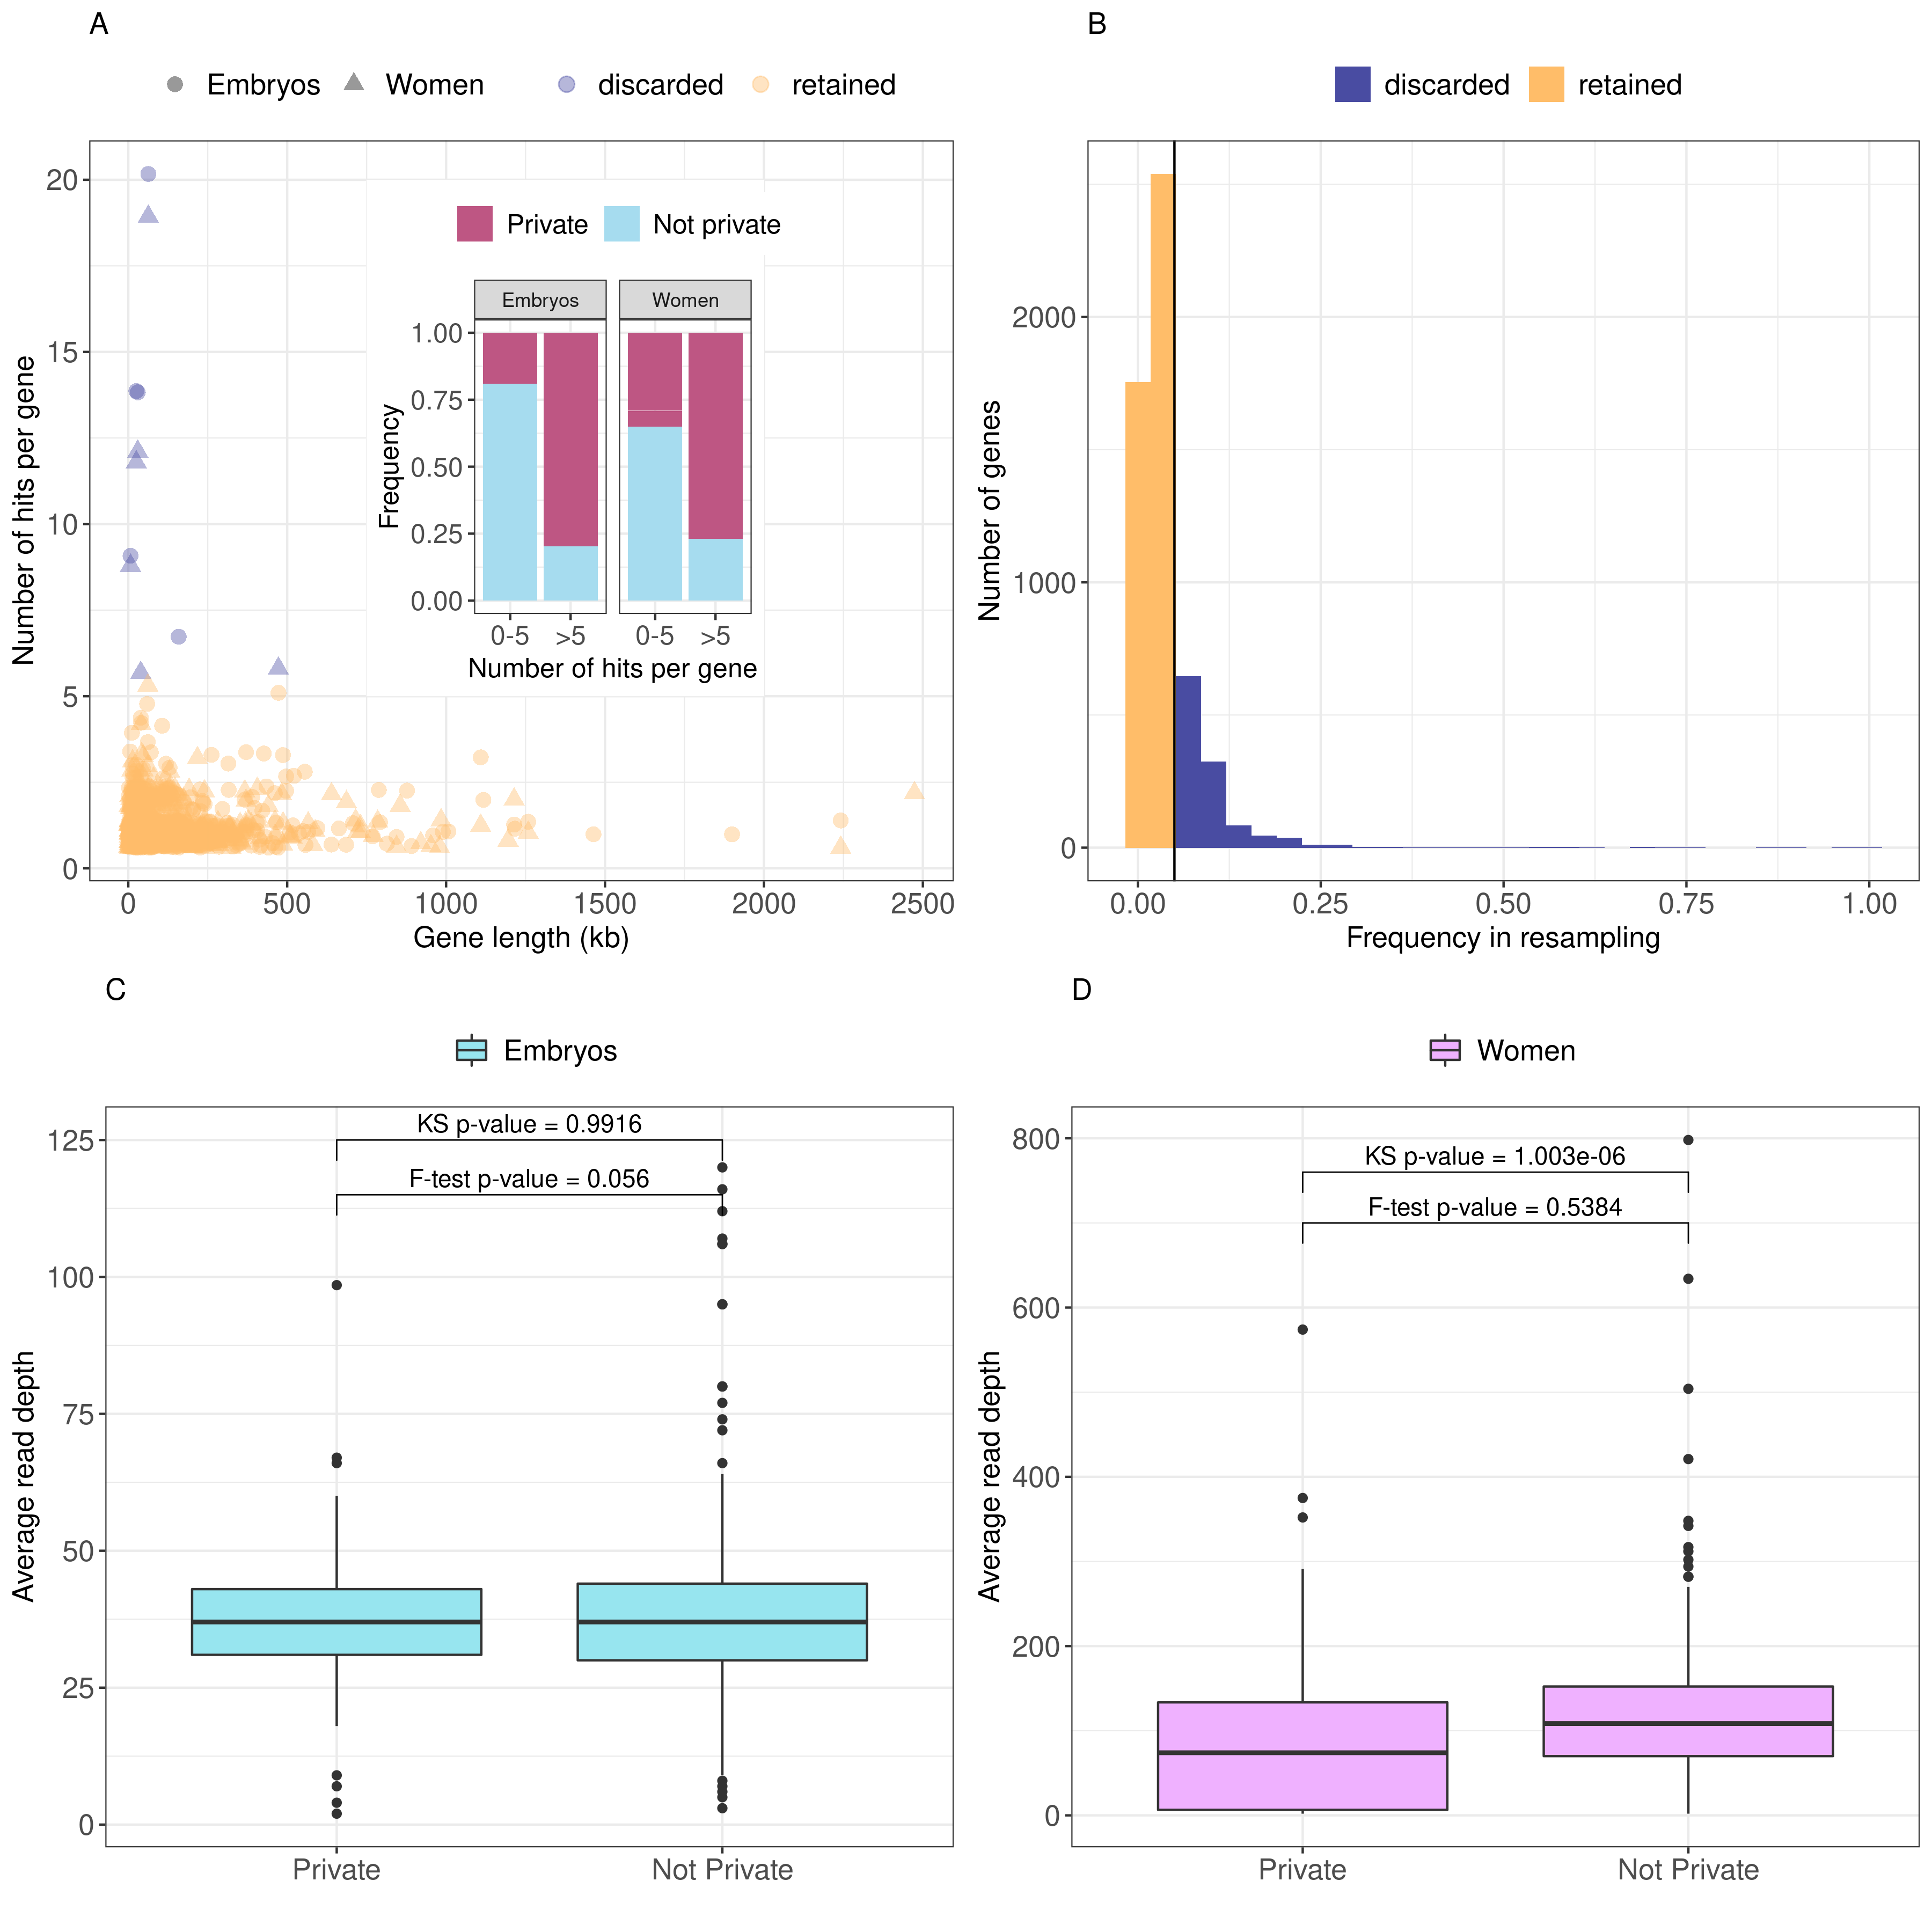
\includegraphics[width=\linewidth]{fig/filters_EmbryoWomen.png}
\caption{\textbf{}}
\label{fig:filters}
\end{figure}

\begin{figure}[ht]
\centering
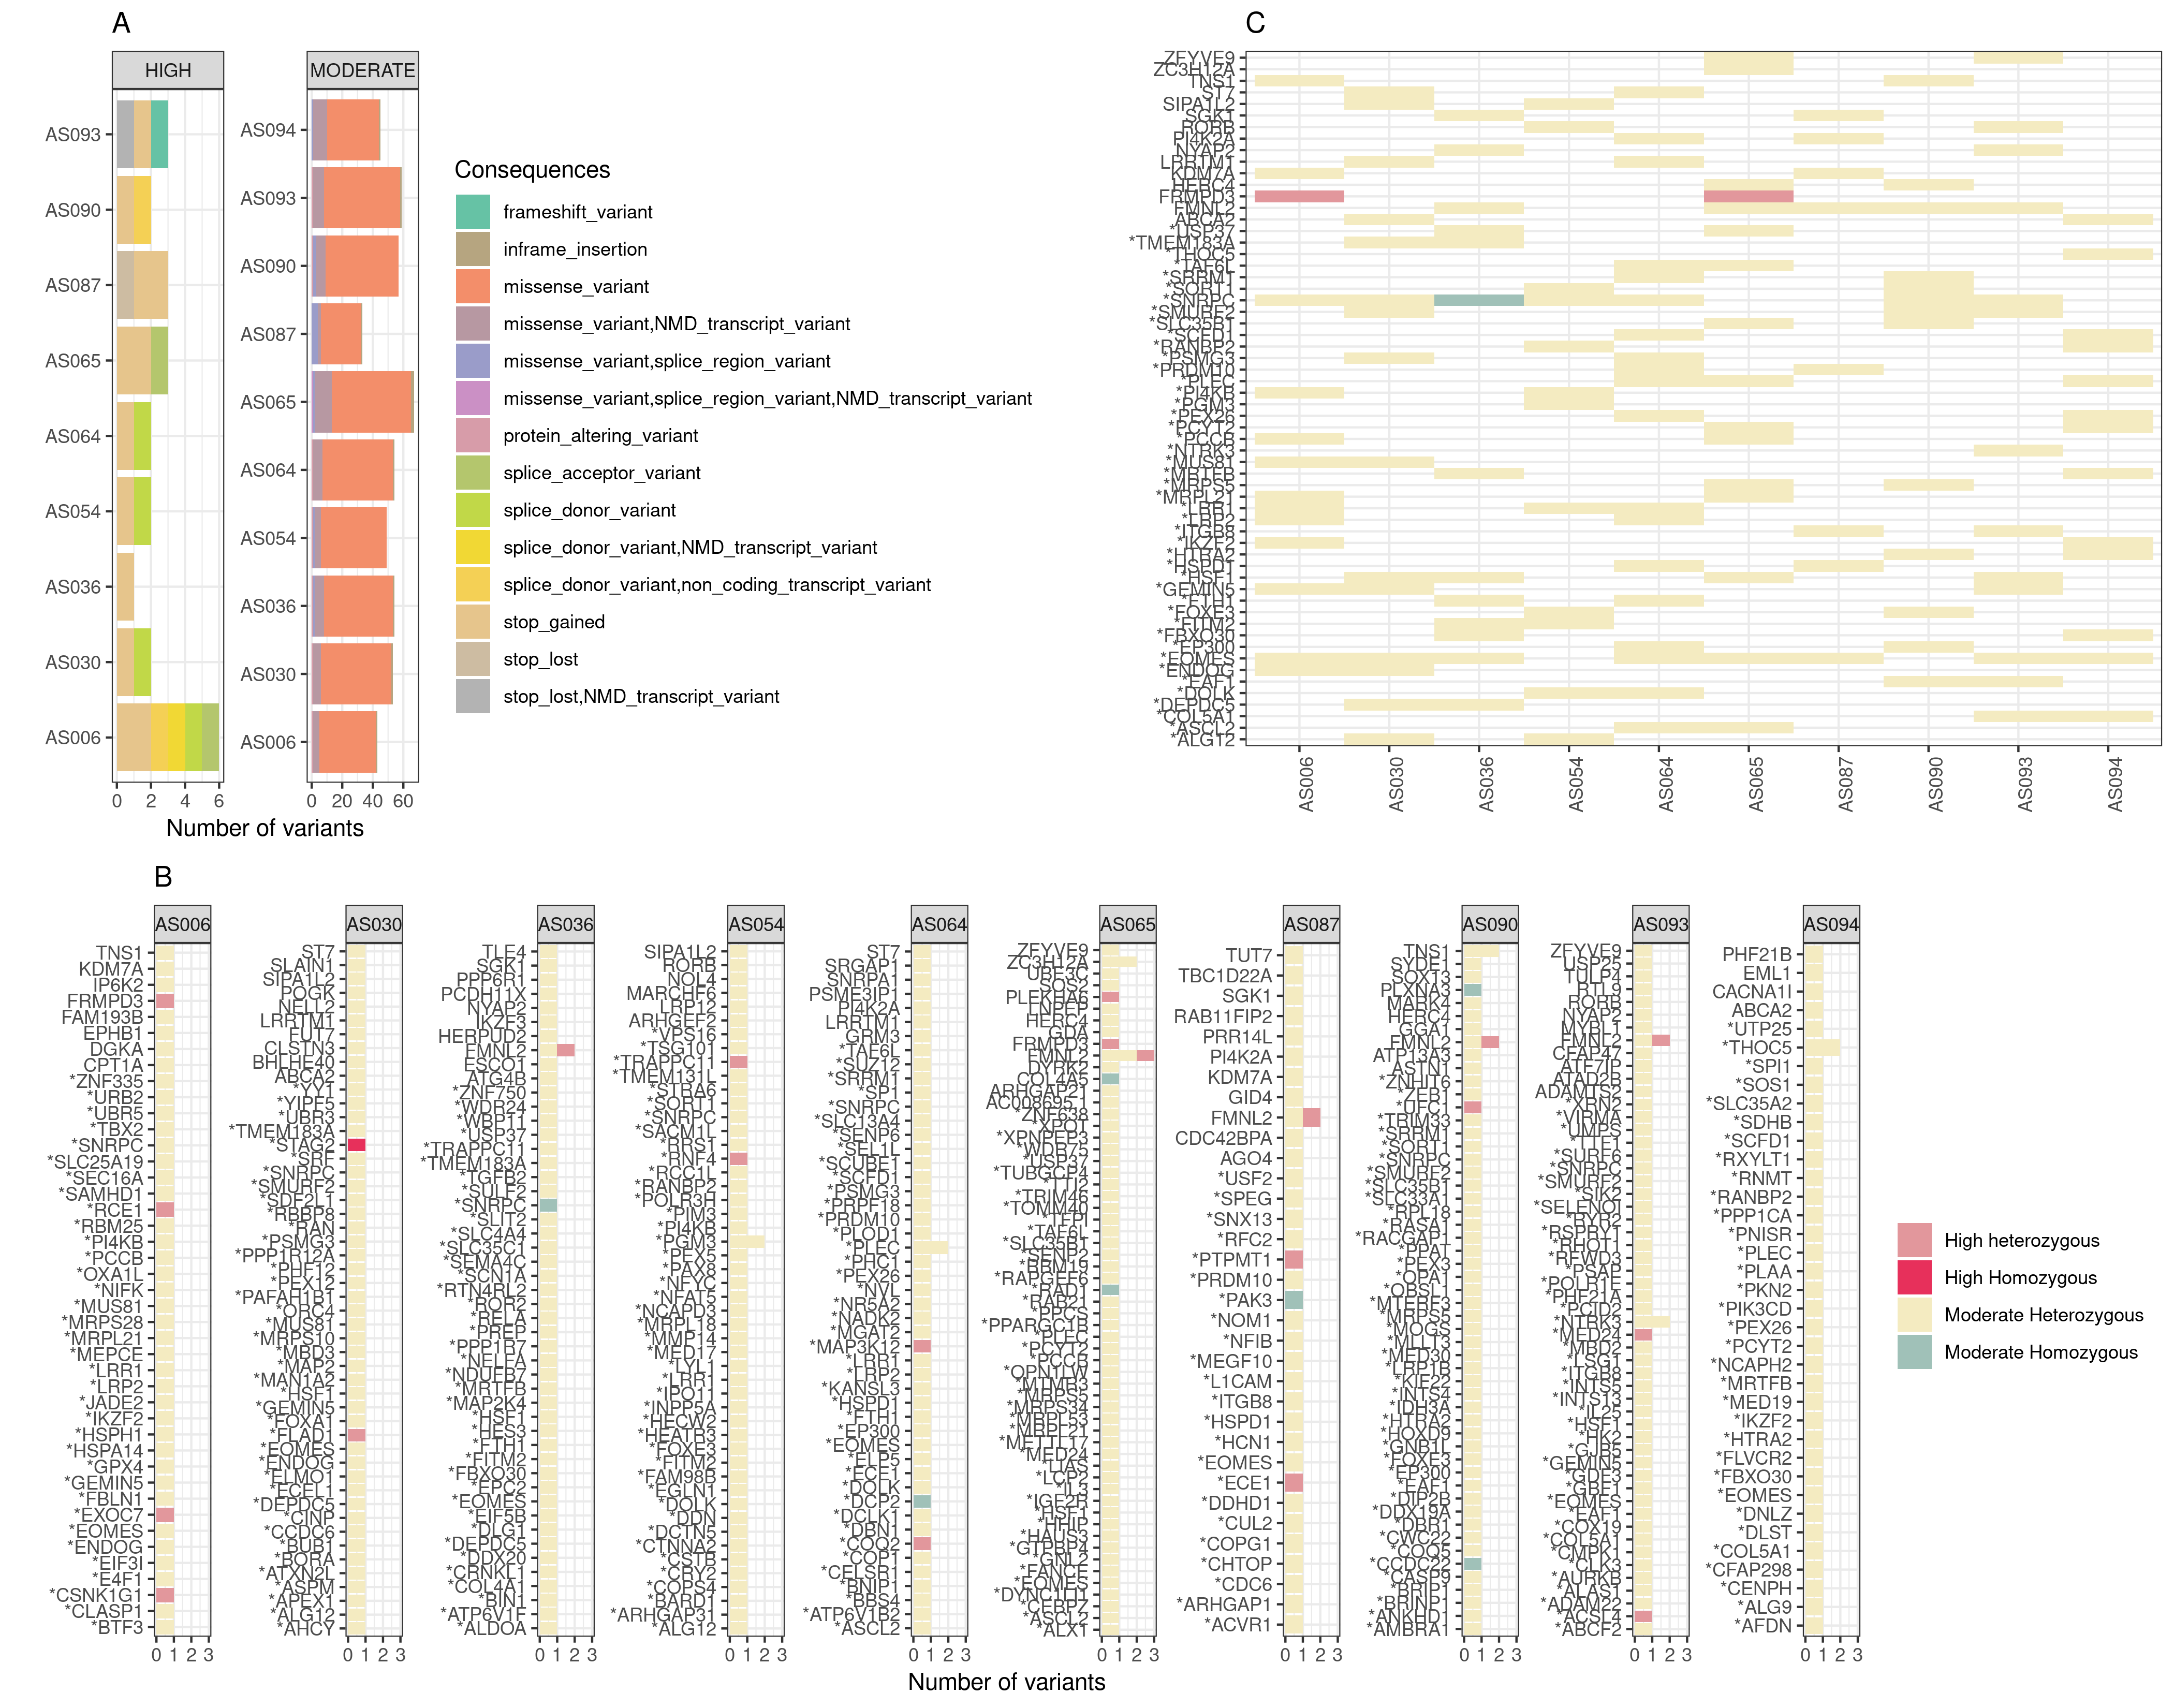
\includegraphics[width=\linewidth]{fig/panel_EmbryoResults.png}
%\caption{\textbf{} he occurrence of variants, their impact, and the count of the consequence allele per gene per embryo  }
\caption{\textbf{}}
\label{fig:resembryo}
\end{figure}

\begin{figure}[ht]
\centering
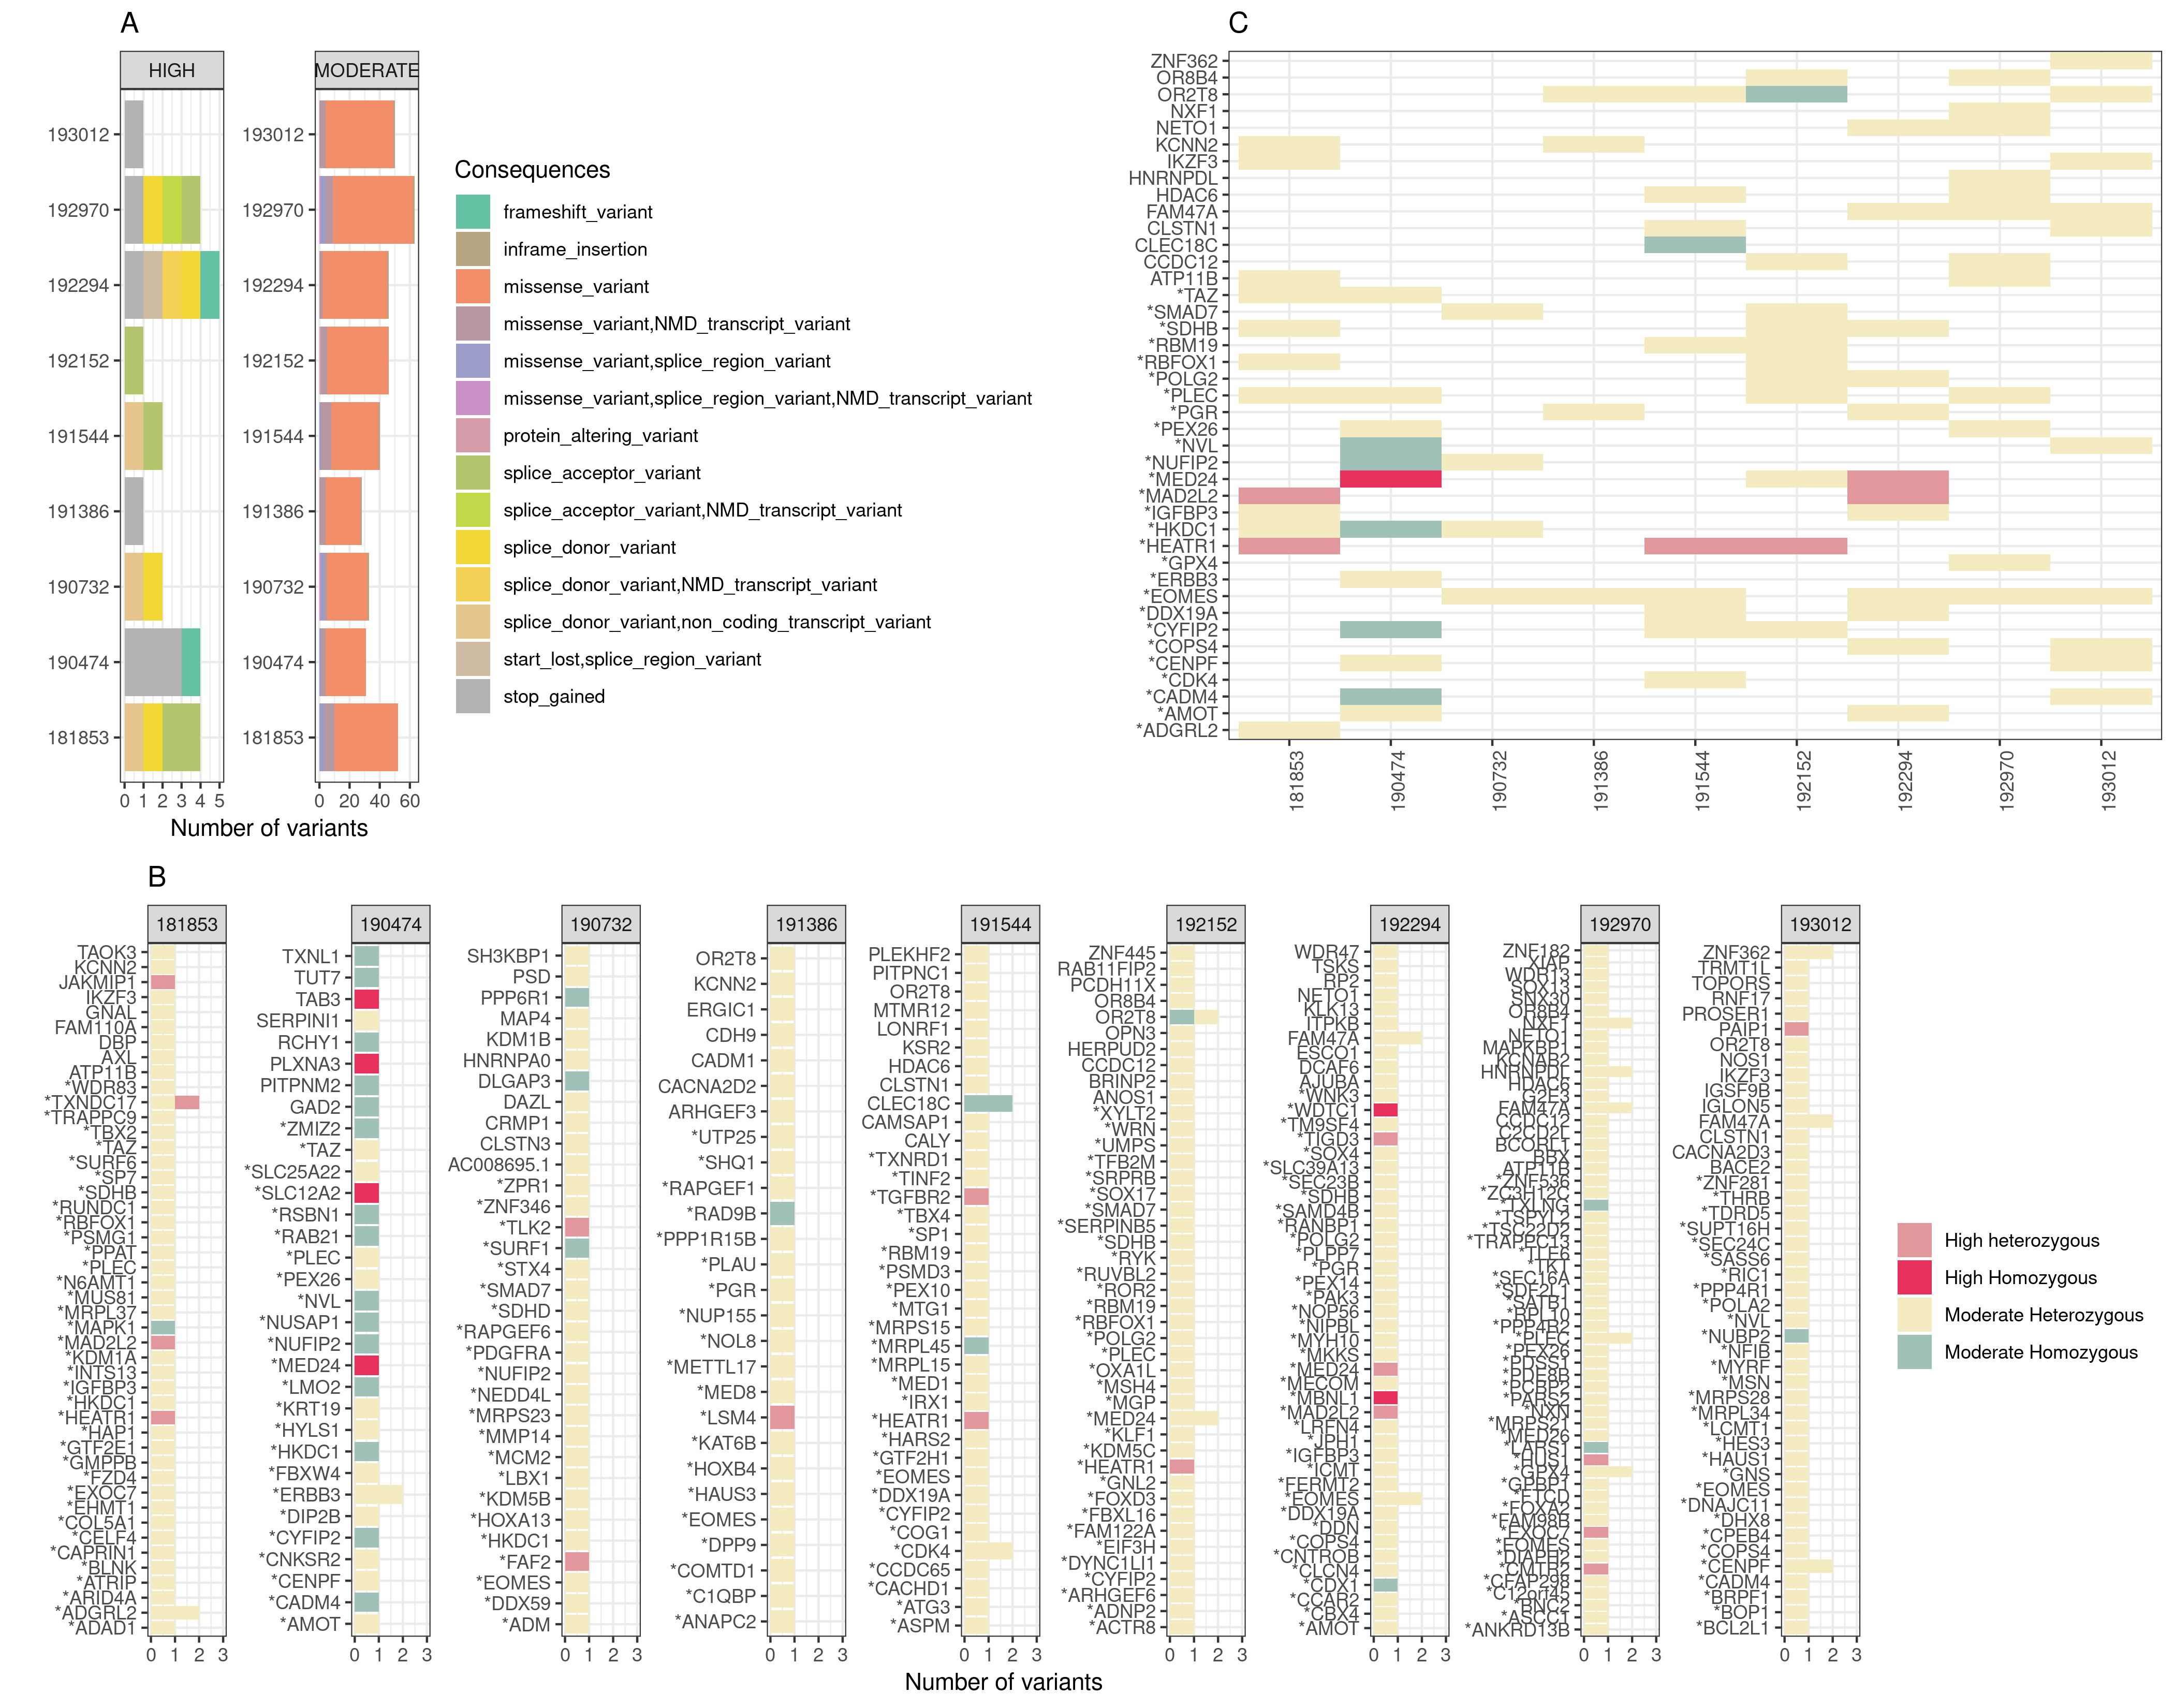
\includegraphics[width=\linewidth]{fig/panel_WomenResults.png}
\caption{\textbf{}  }
\label{fig:reswomen}
\end{figure}

